\section*{Overview}
This technical appendix supports the main paper with the complete pipeline, proofs, protocol, and results.
It is self-contained: it introduces its own notation where needed and refers to no external material.
The material is grouped into five parts.
Appendix~\ref{app:pmethod} specifies the calibration-only algorithm --- the three-stage pipeline, the Fisher--Gram curvature estimator, the interaction-flagged refresh, and the offline cost.
Appendix~\ref{app:ptheory} develops the theory from a compact formal setup: the one-shot quadratic and the revived first-order term derived from the KL risk, the $1/K^2$ step-splitting bound with proof, the exact $K{=}1$ equivalence, one-shot baselines as special cases, and why the flagged refresh suffices.
Appendix~\ref{app:psetup} details the models, baselines, and metrics.
Appendix~\ref{app:presults} reports the full results: per-corpus perplexity, the downstream and generation breakdown, the white-box selection analysis, continuation traces, and the refresh, schedule, anchor, robustness, and efficiency studies.
Appendix~\ref{app:plimits} states scope, limitations, and future work.
Each numbered claim is stated with the assumptions under which it holds, and each table and figure is accompanied by the reading we draw from it.

\section{Method and Algorithm Details}\label{app:pmethod}

\subsection{The \method Pipeline}
\label{app:pipeline}
\method has three offline stages, all calibration-only and gradient-free.
\textbf{(1) Teacher cache.} One forward pass over $\mathcal{C}$ stores, per token, the dense top-$r$
logit indices, probabilities, and logits ($r{=}256$); these fix a common coordinate system in which
every later perturbation is expressed, so all curvatures are anchored to $p_0$.
\textbf{(2) Step-0 ablation.} For every unit $u$ a single masked forward yields the marginal logit
perturbation $\dz_u=z_0-z_{\{u\}}$ on the teacher coordinates; with layer replay this costs $\approx$
one forward per unit, amortized once. \textbf{(3) Continuation.} The continuation traces the
budget path, greedily filling each band by the marginal gain of Eq.~\eqref{eq:marginal} and
re-ablating only flagged units at each of the $K$ steps (Alg.~\ref{alg:refresh}).
Stage (2) is exactly the one-shot pruner's curvature build, so $K{=}1$ reuses it verbatim.

\subsection{The Fisher--Gram Curvature Estimator}
\label{app:estimator}
We never materialize the $V{\times}V$ Fisher. For a token with teacher top-$r$ probabilities
$q\in\R^r$ and a logit perturbation $a\in\R^r$ on those coordinates, the Fisher quadratic form is the
\emph{centered, probability-weighted} inner product
\begin{equation}
a^\top \Fisher^0 a \;=\; \textstyle\sum_i q_i a_i^2-\big(\sum_i q_i a_i\big)^2
\;=\;\norm{\phi(a)}_2^2,
\label{eq:phi}
\end{equation}
where $\phi(a)_i=\sqrt{q_i}\,(a_i-\bar a)$ and $\bar a=\sum_i q_i a_i$ is the probability-weighted
mean. Stacking $\phi(\dz_u)$ over all calibration tokens into a feature matrix
$\Phi_u\in\R^{P\times r}$, the curvature is a Gram product
$\Hmat_{uv}=\tfrac1P\langle\Phi_u,\Phi_v\rangle$ and the drift term is
$g_u=\tfrac1P\langle\Phi_{\Delta},\Phi_u\rangle$ with $\Phi_\Delta=\phi(\Delta z^{(k)})$. Curvature
re-estimation at a moved operating point only recomputes the rows $\Phi_u$ of refreshed units; the
Gram is then a cached matrix product. This is the standard self-distillation Fisher estimator; we restate
it so the cost accounting (App.~\ref{app:cost}) is self-contained.

\begin{algorithm}[t]
\caption{Interaction-Flagged Refresh (step $k>0$)}
\label{alg:refresh}
\textbf{Input}: cached features $\{\Phi_u\}$, last increment $D$, surviving $\mathcal{S}$, fraction $\tau$\\
\textbf{Output}: updated $\Hmat^{(k)},g^{(k)}$
\begin{algorithmic}[1]
\STATE accrue $\sigma_w\!\mathrel{+}=\!\sum_{u\in D}|\Hmat_{wu}|$ for $w\in\mathcal{S}$ \hfill // cumulative since last refresh
\STATE $\mathcal{R}\!\leftarrow$ top-$\tau$ of $\mathcal{S}$ by $\sigma$; $\sigma_w\!\leftarrow\!0$, re-ablate each $w\!\in\!\mathcal{R}$, update $\Phi_w$
\STATE recompute base logits $z_{s_k}$ (one forward); $\Phi_\Delta\!\leftarrow\!\phi(z_0-z_{s_k})$
\STATE $\Hmat^{(k)}\!\leftarrow\!\tfrac1P\Phi\Phi^\top$; $\ g^{(k)}\!\leftarrow\!\tfrac1P\Phi\Phi_\Delta^\top$
\end{algorithmic}
\end{algorithm}

\subsection{Complexity and Offline Cost}
\label{app:cost}
Let $F$ be the cost of one calibration forward and $M$ the number of units. Stage (2) costs $MF$
(layer-replay amortized). Each continuation step re-ablates $\tau|\mathcal{S}|$ units plus one base forward;
over $K$ steps with the first served from cache, the offline cost is
$\big(1+(K{-}1)\tau\big)MF + O(K\cdot F)$, i.e.\ a small constant multiple of one shot
($4.5\times$ at $K{=}8,\tau{=}0.5$). The greedy fill is $O(M^2)$ vector work per step, negligible
next to forwards. \textbf{Deployment cost is unchanged}: \method outputs a mask, so the pruned model's
parameters, FLOPs, and latency are identical to a one-shot model at the same sparsity; the continuation buys
a better mask at the same deployed budget.

\section{Theoretical Analysis}\label{app:ptheory}

\subsection{Setup and notation}
\label{app:setup-theory}
We write $s\in\{0,1\}^U$ for a structured mask over $U$ removable units, $p_s$ for the resulting pruned model, and $c_u$ for the cost of unit $u$.
\method minimizes the calibration KL to the dense teacher $p_0$,
\begin{equation}
\Risk(s)=\E_{x\sim\mathcal{C}}\,\KL\!\big(p_0(\cdot\mid x)\,\|\,p_s(\cdot\mid x)\big),
\label{eq:risk}
\end{equation}
which needs only forward passes.
Expanding \eqref{eq:risk} once at the dense model gives the one-shot second-order surrogate
\begin{equation}
\Risk(s)\approx\tfrac12\,s^\top\Hmat\,s,\qquad \Hmat_{uv}=\E_x\big[\dz_u^\top\Fisher^0\dz_v\big],
\label{eq:oneshot}
\end{equation}
with $\Fisher^0=\mathrm{diag}(p_0)-p_0p_0^\top$ the dense Fisher metric, $z_s$ the logits of $p_s$, and $\dz_u=z_0-z_{\{u\}}$ the marginal logit change of removing $u$ from the dense model.
At a pruned operating point $s_k$ we track the accumulated drift $\Delta z^{(k)}=z_0-z_{s_k}$ and the refreshed marginal perturbations $\dz^{(k)}_u=z_{s_k}-z_{s_k\cup\{u\}}$.
Holding the metric fixed at $\Fisher^0$ but refreshing these perturbations at the current model gives the anchored surrogate
\begin{align}
g^{(k)}_u&=\E_x\big[\Delta z^{(k)\top}\Fisher^0\dz_u^{(k)}\big], \label{eq:grad}\\
\Hmat^{(k)}_{uv}&=\E_x\big[\dz_u^{(k)\top}\Fisher^0\dz_v^{(k)}\big], \label{eq:hess}
\end{align}
and the greedy marginal gain of adding $u$ to the current increment $D$ is
\begin{equation}
\Delta(u\mid D)=\Big(g^{(k)}_u+\tfrac12\Hmat^{(k)}_{uu}+\textstyle\sum_{v\in D}\Hmat^{(k)}_{uv}\Big)\big/c_u.
\label{eq:marginal}
\end{equation}
The \emph{exact} local Taylor coefficients at $s_k$ instead use the moving operating-point Fisher $\Fisher^{(k)}=\mathrm{diag}(p_{s_k})-p_{s_k}p_{s_k}^\top$, namely $\bar g^{(k)}_u=\E_x[(p_0-p_{s_k})^\top\dz^{(k)}_u]$ and $\bar\Hmat^{(k)}_{uv}=\E_x[\dz^{(k)\top}_u\Fisher^{(k)}\dz^{(k)}_v]$, so that $\Risk(s_k{+}\delta)-\Risk(s_k)=\bar g^{(k)\top}\delta+\tfrac12\delta^\top\bar\Hmat^{(k)}\delta+\xi_k(\delta)$; \method\ implements \eqref{eq:grad}--\eqref{eq:hess} in their place, and $\varepsilon_k$ is the resulting per-step gap between the two local quadratics.
Finally, $\norm{x}_{A}\!:=\!\sqrt{x^\top A x}$ is the seminorm induced by a positive-semidefinite matrix $A$, and the \emph{Fisher length} of a path is its arc length in this metric.
The remainder of this part derives \eqref{eq:oneshot}--\eqref{eq:grad} from \eqref{eq:risk} (App.~\ref{app:quad}--\ref{app:firstorder}), proves the step-splitting bound (App.~\ref{app:proof}), and establishes the $K{=}1$ equivalence and the sufficiency of the flagged refresh.

\subsection{The Pruning Quadratic from the KL Risk}
\label{app:quad}
At fixed input, view $\KL(p_0\,\|\,p_z)$ as a function of logits $z$. Its gradient is
$\nabla_z\KL=\mathrm{softmax}(z)-p_0$ and its Hessian is $\mathrm{diag}(\mathrm{softmax}(z))-
\mathrm{softmax}(z)\mathrm{softmax}(z)^\top$. At $z{=}z_0$ the gradient vanishes and the Hessian is the
dense Fisher $\Fisher^0$. A second-order expansion about $z_0$ thus gives
$\KL(p_0\|p_z)\approx\tfrac12(z{-}z_0)^\top\Fisher^0(z{-}z_0)$. Modeling the logit perturbation of a
mask as additive over units, $z_0-z_s=\sum_u s_u\dz_u$, and taking expectations over $\mathcal{C}$
yields $\Risk(s)\approx\tfrac12 s^\top\Hmat s$ with $\Hmat_{uv}=\E[\dz_u^\top\Fisher^0\dz_v]$
(Eq.~\ref{eq:oneshot}). The vanishing gradient \emph{at the dense point} is precisely why one-shot
pruning has no first-order term, a property that does \emph{not} survive once the expansion point
moves.

\subsection{The Revived First-Order Term}
\label{app:firstorder}
At a pruned operating point $s_k$ the expansion point is $z_{s_k}\!\neq\!z_0$, so the KL gradient no
longer vanishes: $\nabla_z\KL(p_0\|p_z)\big|_{z_{s_k}}=p_{s_k}-p_0$. To first order
$p_{s_k}-p_0\approx\Fisher^0(z_{s_k}-z_0)=-\Fisher^0\Delta z^{(k)}$. The additional risk of pruning
$u$ (logit change $-\dz_u^{(k)}$) therefore carries the linear term
$g^{(k)}_u=\E[\Delta z^{(k)\top}\Fisher^0\dz^{(k)}_u]$ (Eq.~\ref{eq:grad}).
\textbf{Zero at the dense model:} $\Delta z^{(0)}{=}0\Rightarrow g^{(0)}{=}0$, recovering
Eq.~\eqref{eq:oneshot}. \textbf{Monotone growth:} $\norm{\Delta z^{(k)}}_{\Fisher^0}^2=2\,\Risk(s_k)$
to second order, which is non-decreasing along the budget; hence the scale of $g^{(k)}$ grows with
sparsity, and a unit whose perturbation aligns with the accumulated drift is penalized. This term is
unavailable to any method whose expansion point coincides with its anchor, and Fig.~\ref{fig:mech}
confirms its predicted growth empirically.

\subsection{Step-splitting: the $1/K^2$ bound}
\label{app:proof}
\begin{proposition}[Step-splitting with surrogate mismatch]\label{prop:k2}
Suppose the exact local Taylor remainder obeys $|\xi_k(\delta_k)|\le L\norm{\delta_k}_{\bar\Hmat^{(k)}}^3$,
and the implemented anchored surrogate $\widehat Q_k(\delta_k)=g^{(k)\top}\delta_k+\tfrac12\delta_k^\top\Hmat^{(k)}\delta_k$
differs from the exact local quadratic $Q_k(\delta_k)=\bar g^{(k)\top}\delta_k+\tfrac12\delta_k^\top\bar\Hmat^{(k)}\delta_k$
by at most $\varepsilon_k$. For a path of total Fisher length $R$ split into $K$ equal-length steps,
\[
\Big|\Risk(s_K)-\Risk(s_0)-\textstyle\sum_{k=0}^{K-1}\widehat Q_k(\delta_k)\Big|\;\le\;\frac{LR^3}{K^2}+\sum_{k=0}^{K-1}\varepsilon_k.
\]
\end{proposition}

\noindent\emph{Proof.} Write the exact additional risk on segment $k$ as
$\Risk(s_k{+}\delta_k)-\Risk(s_k)=Q_k(\delta_k)+\xi_k(\delta_k)$. Summing over the $K$ segments and
subtracting the implemented surrogates, the triangle inequality gives
\[
\begin{aligned}
\Big|\Risk(s_K)-\Risk(s_0)-\textstyle\sum_k\widehat Q_k\Big|
&\le\sum_k|\xi_k(\delta_k)|+\sum_k|Q_k-\widehat Q_k| \\
&\le\sum_k L\norm{\delta_k}_{\bar\Hmat^{(k)}}^3+\sum_k\varepsilon_k .
\end{aligned}
\]
Under equal-Fisher-length steps each segment has length $\le R/K$, and because re-linearization resets the
expansion point the third-order remainders \emph{add} rather than compound:
$\sum_k L\norm{\delta_k}^3\le K\cdot L(R/K)^3=LR^3/K^2$. The mismatch $\varepsilon_k$ collects the effect of
retaining the fixed anchor metric $\Fisher^0$ in place of the exact $\bar\Fisher^{(k)}$ and of the partial
($\tau{<}1$) refresh; it is bounded per step in App.~\ref{app:staleness}. \hfill$\square$

\smallskip\noindent At $K{=}1$ the bound is $LR^3+\varepsilon_0$: the \emph{cubic} growth that, compounded
across the budget, yields the super-exponential collapse. The $1/K^2$ term converts it to additive
degradation; the realized reduction is model-dependent, set by each path's curvature rather than the
worst-case smoothness constant, and is tracked by the per-step predicted/actual ratio $\eta_k$ that
\method logs (App.~\ref{app:fulltrace}).

\textbf{Schedule and the bound.} The partition above uses segments of \emph{equal Fisher length} $R/K$,
which is precisely the \emph{adaptive equal-predicted-risk} schedule of App.~\ref{app:schedule}; under a
convex risk-vs-cost profile this differs from the \emph{equal-cost} default we use in practice. We adopt
equal-cost as a robust, parameter-free surrogate: it needs no per-model risk profiling, the monotone-in-$K$
decay holds empirically under it (Fig.~\ref{fig:kstep}), and the adaptive schedule that \emph{does} match
the bound's premise reproduces the front-loaded gain on the sharpest-collapsing models
(App.~\ref{app:schedule}). The $1/K^2$ rate is therefore the geometry the theorem predicts; the equal-cost
default trades a tighter worst-case constant for robustness, with the realized reduction set by each
model's path curvature rather than the uniform-smoothness constant. The bound further assumes \emph{exact}
re-linearization at each step; the flagged refresh ($\tau{<}1$) re-estimates only the units whose curvature
is expected to move, and the residual staleness this leaves is bounded separately in
App.~\ref{app:staleness}.

\subsection{$K{=}1$ Equivalence}
\label{app:k1}
With $K{=}1$ the single band spans $[0,B]$ and the only estimate is at $s_0{=}\mathbf 0$, where
$\Delta z^{(0)}{=}0$, $g^{(0)}{=}0$, and $\Hmat^{(0)}{=}\Hmat$ is the dense Gram. The greedy of
Eq.~\eqref{eq:marginal} then minimizes $\tfrac12\delta^\top\Hmat\delta$ subject to the budget, exactly
the one-shot second-order pruner. We verify this equivalence numerically: at $K{=}1$ the two produce
bit-level-identical selected sets (Jaccard $1.0$). Thus any gap between \method and one-shot is attributable solely to
path refinement, not to a different objective, estimator, or unit substrate.

\subsection{One-Shot Baselines as Special Cases}
\label{app:special}
Equation~\eqref{eq:oneshot} subsumes the calibration-only baselines as approximations of $\Hmat$ at
$k{=}0$: \emph{magnitude} drops the data and uses $\|\theta_u\|$; \emph{Taylor saliency}
\citep{molchanov2019taylor,ma2023llmpruner} keeps the diagonal $g{+}\tfrac12\Hmat_{uu}$ at the dense
point; \emph{Wanda} \citep{sun2024wanda} replaces $\Hmat_{uu}$ by a weight$\times$activation
surrogate; \emph{activation-fluctuation} \citep{an2024flap} uses a variance statistic in place of the
Fisher quadratic. All share the defining one-shot move, a single estimate at the anchor, so all
inherit the collapse (App.~\ref{app:percorpus}).

\subsection{Why Interaction-Flagged Refresh Suffices}
\label{app:staleness}
When increment $D$ is pruned, a surviving unit $w$'s feature changes by
$\Delta\Phi_w=\phi(\dz_w^{(k{+}1)})-\phi(\dz_w^{(k)})$, driven by the operating-point shift along
$\{\dz_u\}_{u\in D}$. To first order this shift couples $w$ to $D$ through the off-diagonal curvature,
so $\norm{\Delta\Phi_w}\lesssim c\sum_{u\in D}|\Hmat^{(k)}_{wu}|$ for a constant $c$ absorbing the
local third-order scale. Units with negligible interaction to $D$ have near-unchanged curvature and
may safely reuse cached features; refreshing the top-$\tau$ by the \emph{cumulative}
$\sigma_w=\sum_{j}\sum_{u\in D_j}|\Hmat_{wu}|$ (over all bands $D_j$ since $w$'s last refresh)
captures the largest accumulated changes first, so no survivor stays stale indefinitely. The refresh fraction $\tau$ thus trades offline cost for
estimation fidelity; the ablation grid (App.~\ref{app:ablation}) shows too small a $\tau$ leaves stale
curvature that re-introduces the one-shot pathology, fixing $\tau{=}0.5$ as the default.

\section{Experimental Setup and Implementation}\label{app:psetup}

\subsection{Models and Protocol}
\label{app:setup}
\paragraph{Models.} Seven open dense decoder-only LLMs spanning five families and three scales:
LLaMA-2-7B~\citep{touvron2023llama2}, LLaMA-3.1-8B and LLaMA-3.2-3B~\citep{dubey2024llama3},
Qwen2.5-7B and Qwen2.5-14B~\citep{qwen2025qwen25}, Yi-1.5-9B~\citep{ai2024yi}, and
Falcon3-7B~\citep{falcon3} (Table~\ref{tab:models}).

\paragraph{Structural units and cost.} Attention heads are grouped KV-aligned; FFN units are contiguous
intermediate-channel groups (16 per layer); the cost $c_u$ of a unit is its parameter count.

\paragraph{Calibration.} 48 sequences $\times$ 512 tokens from a C4/WikiText mix, held fixed and
identical for every method.

\paragraph{Safety rails (shared by all methods).} A protected band (first/last 2 layers) and an adaptive
per-layer cap $\mathrm{cap}(\rho)=\min(0.85,\rho{+}0.2)$ --- loose enough to reach the global target yet
preventing any single layer from being emptied. Reported for fairness and applied identically to every method.

\paragraph{Structural removal.} Selected units are physically deleted (heads dropped, FFN sliced), so the
reported efficiency is real and the logit error versus runtime masking is zero.

\paragraph{\method{} configuration.} Equal budget bands; $\tau{=}0.5$ and $K{=}8$ by default
($K\in\{1,2,4\}$ in the ablation); the first step is served from the dense cache. The three-seed
robustness study (App.~\ref{app:robustness}) redraws the calibration set with seeds $\{0,1,2\}$; all
other results use seed $0$.

\begin{table}[t]\centering\footnotesize
\caption{Models and structural-unit inventory. Heads are counted as KV-aligned groups (GQA models
have fewer KV heads than query heads); FFN groups are contiguous intermediate-channel blocks.}
\label{tab:models}
\setlength{\tabcolsep}{4pt}
\begin{tabular}{l c c c c c}
\toprule
Model & Attn. & KV heads & FFN grp & Layers & Units $M$ \\
\midrule
LLaMA-2-7B   & MHA & 32 & 16 & 32 & 1536 \\
LLaMA-3.1-8B & GQA & 8  & 16 & 32 & 768 \\
LLaMA-3.2-3B & GQA & 8  & 16 & 28 & 672 \\
Qwen2.5-7B   & GQA & 4  & 16 & 28 & 560 \\
Qwen2.5-14B  & GQA & 8  & 16 & 48 & 1152 \\
Yi-1.5-9B    & GQA & 4  & 16 & 48 & 960 \\
Falcon3-7B   & GQA & 4  & 16 & 28 & 560 \\
\bottomrule
\end{tabular}
\end{table}

\subsection{Baseline Descriptions and Configuration}
\label{app:baselines}
\paragraph{Selection-only baselines.}
All are run from their official implementations under one shared protocol (same calibration set, caps, and protected band; per-method settings in Table~\ref{tab:hparams}).
\emph{One-shot} ($K{=}1$) is \method with a single step, the exact dense-point second-order pruner of Eq.~\eqref{eq:oneshot}.
\emph{Wanda-sp}~\citep{sun2024wanda} uses a weight$\times$activation norm; \emph{FLAP}~\citep{an2024flap} an activation-fluctuation criterion; \emph{LLM-Pruner}~\citep{ma2023llmpruner} grouped Taylor saliency (LoRA disabled for the main comparison, with native LoRA recovery reported separately).
\emph{Magnitude} and \emph{random} are cost-normalized lower bounds.
Our one-shot is the exact $K{=}1$ case of \method, and Wanda-sp/FLAP reproduce their published low-sparsity perplexities; the large high-sparsity values (e.g.\ FLAP at $\rho{=}0.5$) are the genuine no-recovery behavior of these criteria once retraining is removed --- not a misconfiguration, but the collapse this paper characterizes.

\paragraph{FLAP's bias compensation.}
FLAP additionally replaces each pruned channel by its calibration mean, adding a constant bias $W\mu_{\text{rm}}$ to the next projection.
This is a mask-agnostic, label-free correction, orthogonal to selection and composable with \emph{any} mask (including \method's), so we disable it for all methods in the main comparison and report it as an add-on applied identically to every mask (App.~\ref{app:efficiency}).

\paragraph{Reconstruction-based references (LLM Surgeon, SlimGPT, SlimLLM).}
These \emph{update the surviving weights} as an integral part of the method --- multi-shot correlated OBS updates plus optional LoRA (LLM Surgeon~\citep{ouderaa2024llmsurgeon}), grouped OBS updates (SlimGPT~\citep{ling2024slimgpt}), and a least-squares output-matrix refit (SlimLLM~\citep{guo2025slimllm}) --- which places them on a different axis from \method's zero-update selection.
To compare selection alone, we run the two structured layer-wise pruners under our no-update protocol (reconstruction disabled).
Stripped of reconstruction both collapse at high sparsity, \emph{below even one-shot} (Table~\ref{tab:allbaselines}: SlimGPT reaches WikiText $15.4$k/$104$k on LLaMA-2-7B/3.1-8B, SlimLLM $7107$ on LLaMA-2-7B at $\rho{=}0.5$), so their reported quality is the value of reconstruction, not of selection.
Refitting the surviving weights does reach lower absolute perplexity than any weight-frozen method, ours included; but that gap measures reconstruction, and reconstruction operates \emph{on top of} a mask, so a higher-quality mask only helps it.
Even so, structured LLM Surgeon is near-lossless only to $20$--$30\%$, its higher-sparsity points relying on the weight updates: in the strictly weight-frozen regime we isolate, \emph{no} method avoids the collapse.

\paragraph{Why selection is the upstream axis.}
Disabling all recovery (LoRA, fine-tuning, reconstruction) isolates a single question --- \emph{which units to remove} --- and matches the standard headline setting for training-free pruners, which report main results without retraining (SliceGPT~\citep{ashkboos2024slicegpt}, FLAP~\citep{an2024flap}, SparseGPT~\citep{frantar2023sparsegpt}, Wanda~\citep{sun2024wanda}).
Recovery is an orthogonal stage applied on top of a fixed mask, and the papers reporting with/without-recovery pairs (LLM-Pruner~\citep{ma2023llmpruner}, SlimGPT~\citep{ling2024slimgpt}, Bonsai~\citep{dery2024bonsai}) find it lifts every method \emph{without inverting the selection ordering}: LLM-Pruner keeps Taylor selection above magnitude/random both before and after LoRA (a roughly uniform $+2.5$/$+6.5$ point lift at $\rho{=}0.2$/$0.5$), and FLAP's rank-1 bias compensation does not let a weaker selection overtake a stronger one.
A higher-quality mask is therefore the upstream determinant of post-recovery quality, and the selection-only gaps we report bound from below what survives recovery.
We do not claim recovery closes the gap to zero, only that a low-rank adapter is unlikely to invert an ordering as large as the $16.8\times$ perplexity gap at $\rho{=}0.5$.

\begin{table}[t]\centering\footnotesize
\caption{\textbf{Hyperparameter configuration} for \method and the evaluation protocol. A single setting
is used for all seven models with no per-model tuning.}
\label{tab:hparams}
\begin{tabular}{l l}
\toprule
Component & Setting \\
\midrule
Calibration & 48 seq $\times$ 512 tok, C4/WikiText \\
Teacher top-$r$ & 256 \\
\method steps $K$ & 8 (default); 1,2,4 in ablation \\
Refresh $\tau$ & 0.5 \\
Budget schedule & equal \\
Per-layer cap & $\min(0.85,\rho{+}0.2)$ \\
Protected band & first/last 2 layers \\
Eval: ppl stride / seq & 512 / 2048 \\
Eval: generation cap & 256 samples \\
\bottomrule
\end{tabular}
\end{table}

\subsection{Metric Definitions}
\label{app:metrics}
\textbf{Perplexity} on WikiText-2/PTB/C4 with a 2048-token window, stride 512.
\textbf{KL-to-teacher} is Eq.~\eqref{eq:risk} estimated on held-out calibration text, a recovery-free,
task-agnostic distance to the dense model. \textbf{Zero-shot accuracy} (length-normalized) on the
seven commonsense tasks via the LM-Eval-Harness; \textbf{MMLU} zero-shot (length-normalized
log-likelihood over the four options); \textbf{GSM8K} exact-match,
\textbf{HumanEval}/\textbf{MBPP} pass@1 (generation capped at 256 samples, 256 new tokens).
\textbf{Efficiency}: parameter reduction, prefill/decode throughput, and peak memory under structural
removal on a single GPU, measured in a contention-free run.

\section{Full Results and Analysis}\label{app:presults}

\subsection{Per-Corpus Perplexity, All Models}
\label{app:percorpus}
The collapse-and-control pattern holds on \emph{every} corpus and model. Table~\ref{tab:c4} reports
C4 perplexity (one-shot vs.\ \method $K{=}8$); WikiText is in the main paper.
\AppNote{The collapse-and-control pattern is corpus-independent: it holds identically on C4 (below),
WikiText-2 (main results), and the out-of-distribution PTB reported for the headline models in
App.~\ref{app:robustness}.}
\begin{table}[h]\centering\footnotesize
\setlength{\tabcolsep}{3.0pt}
\caption{C4 perplexity ($\downarrow$), one-shot vs.\ \method ($K{=}8$), no recovery, all seven models.
\method is best in every cell.}
\label{tab:c4}
\begin{tabular}{l l cccc}
\toprule
Model & Method & $\rho{=}0.2$ & $\rho{=}0.3$ & $\rho{=}0.4$ & $\rho{=}0.5$ \\
\midrule
\multirow{2}{*}{LLaMA-2-7B}
 & One-shot & 13.6 & 27.8 & 116.7 & 2095 \\
 & \cellcolor{cfhi}\method & \cellcolor{cfhi}\best{11.5} & \cellcolor{cfhi}\best{19.8} & \cellcolor{cfhi}\best{36.9} & \cellcolor{cfhi}\best{337} \\
\midrule
\multirow{2}{*}{LLaMA-3.1-8B}
 & One-shot & 23.6 & 49.3 & 268.0 & 2308 \\
 & \cellcolor{cfhi}\method & \cellcolor{cfhi}\best{19.6} & \cellcolor{cfhi}\best{32.9} & \cellcolor{cfhi}\best{60.7} & \cellcolor{cfhi}\best{211} \\
\midrule
\multirow{2}{*}{LLaMA-3.2-3B}
 & One-shot & 27.9 & 65.3 & 315.9 & 2107 \\
 & \cellcolor{cfhi}\method & \cellcolor{cfhi}\best{22.1} & \cellcolor{cfhi}\best{40.8} & \cellcolor{cfhi}\best{102.9} & \cellcolor{cfhi}\best{261} \\
\midrule
\multirow{2}{*}{Qwen2.5-7B}
 & One-shot & 26.4 & 44.8 & 109.6 & 342.3 \\
 & \cellcolor{cfhi}\method & \cellcolor{cfhi}\best{20.6} & \cellcolor{cfhi}\best{30.9} & \cellcolor{cfhi}\best{60.3} & \cellcolor{cfhi}\best{207} \\
\midrule
\multirow{2}{*}{Qwen2.5-14B}
 & One-shot & 19.3 & 34.4 & 92.7 & 346.2 \\
 & \cellcolor{cfhi}\method & \cellcolor{cfhi}\best{14.7} & \cellcolor{cfhi}\best{22.2} & \cellcolor{cfhi}\best{46.6} & \cellcolor{cfhi}\best{163} \\
\midrule
\multirow{2}{*}{Yi-1.5-9B}
 & One-shot & 308.6 & 1805 & 5420 & 16504 \\
 & \cellcolor{cfhi}\method & \cellcolor{cfhi}\best{13.3} & \cellcolor{cfhi}\best{22.7} & \cellcolor{cfhi}\best{46.3} & \cellcolor{cfhi}\best{88.9} \\
\midrule
\multirow{2}{*}{Falcon3-7B}
 & One-shot & 16.8 & 24.4 & 43.0 & 109.6 \\
 & \cellcolor{cfhi}\method & \cellcolor{cfhi}\best{15.1} & \cellcolor{cfhi}\best{19.6} & \cellcolor{cfhi}\best{28.8} & \cellcolor{cfhi}\best{53.5} \\
\bottomrule
\end{tabular}
\end{table}

\textbf{Lower envelope of the full baseline set, all seven models.} The main text runs the complete
selection-only baseline sweep at every ratio on LLaMA-3.1-8B and LLaMA-2-7B
(Table~\ref{tab:l2degrade}); Table~\ref{tab:allbaselines} confirms that at the high-sparsity operating
point ($\rho{=}0.5$) \method is the lower envelope of \emph{every} training-free baseline on \emph{all
seven} models. The collapse is shared by every score (activation-, weight-, and gradient-based), which is
the paradigm claim of the main paper; \method is the only method that keeps every model out of
the four-to-five-figure regime.

\begin{table*}[t]\centering\footnotesize
\setlength{\tabcolsep}{5.5pt}\renewcommand{\arraystretch}{1.06}
\caption{\textbf{Full selection-only baseline sweep at $\rho{=}0.5$} (WikiText-2 ppl $\downarrow$, no
recovery, all seven models). This includes the \emph{selection criteria} of the reconstruction-based
SOTA, SlimGPT$^\ddagger$ and SlimLLM$^\ddagger$, run in our harness with their weight reconstruction
\emph{disabled} (as for every method here), which isolates selection. Stripped of reconstruction, both
collapse at high sparsity, below even one-shot, confirming that their reported quality comes from the
reconstruction stage (orthogonal to, and composable with, a better mask), not from selection. \method is
the lower envelope on every model. $k{=}10^3$; ``$-$''\,=\,not run (weak baseline already dominated, or
LLM-Pruner/SlimLLM not evaluated at that model). \best{Best}. $^\ddagger$With reconstruction these methods
reach lower absolute ppl; see App.~\ref{app:baselines}.}
\label{tab:allbaselines}
\begin{tabular}{l cccc c c c c c}
\toprule
Model & Rand. & Magn. & Wanda & FLAP & SlimGPT$^\ddagger$ & SlimLLM$^\ddagger$ & LLM-Pr. & 1-shot & \method \\
\midrule
LLaMA-2-7B    & 10.0k & 27.8k & 9124 & 17.6k & 15.4k & 7107 & 686 & 1497 & \cellcolor{cfhi}\best{389} \\
LLaMA-3.1-8B  & 60.4k & 76.3k & 17.6k & 376k & 104k & $-$ & 718 & 4106 & \cellcolor{cfhi}\best{245} \\
LLaMA-3.2-3B  & $-$ & $-$ & 2854 & 65.2k & 80.5k & $-$ & 2491 & 3027 & \cellcolor{cfhi}\best{325} \\
Qwen2.5-7B    & 6894 & 1725 & 830 & 590 & 516 & $-$ & 684 & 270 & \cellcolor{cfhi}\best{141} \\
Qwen2.5-14B   & $-$ & $-$ & 924 & 929 & 573 & $-$ & $-$ & 301 & \cellcolor{cfhi}\best{156} \\
Yi-1.5-9B     & $-$ & $-$ & 16.1k & 13.2k & 48.0k & $-$ & 653 & 16.5k & \cellcolor{cfhi}\best{62} \\
Falcon3-7B    & $-$ & $-$ & 533 & 321 & 194 & $-$ & 52 & 63 & \cellcolor{cfhi}\best{28} \\
\bottomrule
\end{tabular}
\end{table*}

\begin{figure}[t]
\centering
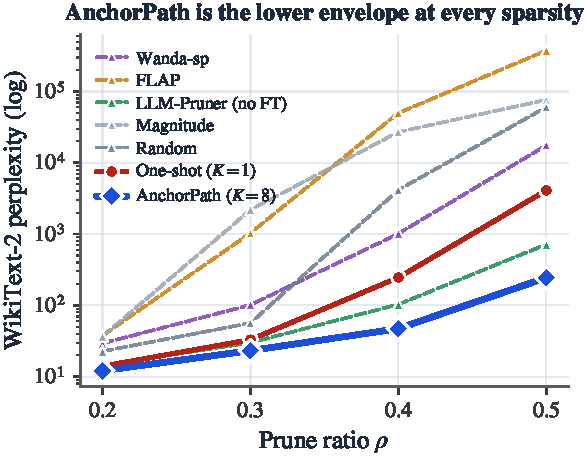
\includegraphics[width=0.94\columnwidth]{figs/fig_baselines.pdf}
\caption{\textbf{\method is the lower envelope of the training-free degradation curve} (companion to the main results table;
LLaMA-3.1-8B, WikiText-2 ppl vs.\ prune ratio, all calibration-only / no recovery).
Activation baselines (Wanda-sp, FLAP) and magnitude diverge by $\rho{=}0.3$; gradient LLM-Pruner is
strongest among external baselines, yet \method ($K{=}8$) is below every method at every sparsity.}
\label{fig:baselines}
\end{figure}

\subsection{Full Zero-Shot, Knowledge, and Generation Breakdown}
\label{app:breakdown}

\textbf{Extended frontier ($\rho{=}0.6/0.7$).} Table~\ref{tab:frontier} backs the extended-sparsity
numbers quoted in the main paper. The multiplier over one-shot keeps growing with sparsity through
$\rho{=}0.6$ (up to $119\times$ on the fragile Yi-1.5-9B); by $\rho{=}0.7$ absolute perplexity is unusable
for \emph{all} calibration-only pruners, yet the continuation still leads one-shot on every model.

\begin{table}[h]\centering\footnotesize
\setlength{\tabcolsep}{5pt}\renewcommand{\arraystretch}{1.06}
\caption{\textbf{Extended sparsity frontier} (WikiText-2 ppl $\downarrow$, $K{=}8$ equal-cost vs.\ one-shot,
no recovery). $k{=}10^3$. The gain over one-shot at $\rho{=}0.6$ is $24.5\times$/$24.1\times$/$119\times$
on LLaMA-2-7B/LLaMA-3.1-8B/Yi-1.5-9B; at $\rho{=}0.7$ no calibration-only method is deployable, but the
continuation still leads one-shot on every model. \best{Best}.}
\label{tab:frontier}
\resizebox{\columnwidth}{!}{%
\begin{tabular}{l cc cc}
\toprule
& \multicolumn{2}{c}{$\rho{=}0.6$} & \multicolumn{2}{c}{$\rho{=}0.7$} \\
\cmidrule(lr){2-3}\cmidrule(lr){4-5}
Model & One-shot & \method & One-shot & \method \\
\midrule
LLaMA-2-7B    & 64.8k & \best{2640} & 74.1k & \best{43.2k} \\
LLaMA-3.1-8B  & 32.6k & \best{1354} & 350k  & \best{13.0k} \\
Yi-1.5-9B     & 56.2k & \best{471}  & 177k  & \best{50.6k} \\
\bottomrule
\end{tabular}}
\end{table}

\AppNote{The full seven-task commonsense breakdown for the canonical LLaMA-2-7B is in
Table~\ref{tab:downstream}, three further models' averages in Table~\ref{tab:dsbreadth}, and
generation (GSM8K/MBPP) in Table~\ref{tab:generation}.}

\textbf{Downstream breadth beyond the main-text three.} The main text reports the 7-task zero-shot average
for LLaMA-3.1-8B, Yi-1.5-9B, and Qwen2.5-7B (condensed in the main paper); Table~\ref{tab:dsbreadth}
extends the comparison to three further models, where \method again lifts the downstream average above its
own one-shot case at every measured ratio, confirming the accuracy gain is a property of the continuation
rather than of a particular architecture.

\begin{table}[h]\centering\footnotesize
\setlength{\tabcolsep}{6pt}\renewcommand{\arraystretch}{1.05}
\caption{\textbf{Downstream gain on three further models} (7-task zero-shot avg.\ $\uparrow$, no recovery).
\method ($K{=}8$, equal bands) vs.\ its own one-shot case. Best per row. (Qwen2.5-14B/Falcon3 zero-shot at
$\rho{=}0.3$ not run; LLM-Pruner not evaluated at 14B, its other cross-model cells are in
the main paper.)}
\label{tab:dsbreadth}
\begin{tabular}{l c cc}
\toprule
Model & $\rho$ & One-shot & \method \\
\midrule
\multirow{3}{*}{LLaMA-3.2-3B}
 & 0.3 & .458 & \cellcolor{cfhi}\best{.470} \\
 & 0.4 & .411 & \cellcolor{cfhi}\best{.429} \\
 & 0.5 & .372 & \cellcolor{cfhi}\best{.411} \\
\midrule
\multirow{2}{*}{Qwen2.5-14B}
 & 0.4 & .471 & \cellcolor{cfhi}\best{.507} \\
 & 0.5 & .420 & \cellcolor{cfhi}\best{.430} \\
\midrule
\multirow{2}{*}{Falcon3-7B}
 & 0.4 & .471 & \cellcolor{cfhi}\best{.485} \\
 & 0.5 & .406 & \cellcolor{cfhi}\best{.455} \\
\bottomrule
\end{tabular}
\end{table}

\begin{table}[t]\centering\footnotesize
\setlength{\tabcolsep}{5pt}\renewcommand{\arraystretch}{1.06}
\caption{\textbf{Generation collapses for every no-recovery pruner} (GSM8K exact-match \%, no recovery).
Dense models score in double digits, but at $\rho{=}0.3$--$0.5$ every calibration-only method falls to
noise level ($\lesssim2\%$); MBPP pass@1 behaves identically. The collapse is a property of the regime, not
of any one selection criterion, and is restored by the orthogonal recovery stage.}
\label{tab:generation}
\begin{tabular}{l cc cc}
\toprule
& \multicolumn{2}{c}{LLaMA-2-7B} & \multicolumn{2}{c}{LLaMA-3.1-8B} \\
\cmidrule(lr){2-3}\cmidrule(lr){4-5}
Method (no recovery) & $\rho{=}0.3$ & $\rho{=}0.5$ & $\rho{=}0.3$ & $\rho{=}0.5$ \\
\midrule
One-shot ($K{=}1$) & 1.6 & 0.0 & 1.2 & 0.1 \\
LLM-Pruner & 0.4 & 0.0 & 2.2 & 0.2 \\
\method ($K{=}8$) & 0.8 & 0.4 & 1.7 & 0.2 \\
\bottomrule
\end{tabular}
\end{table}

\begin{table*}[t]
\centering\footnotesize
\setlength{\tabcolsep}{4.6pt}\renewcommand{\arraystretch}{1.06}
\caption{\textbf{Detailed downstream zero-shot accuracy on the canonical LLaMA-2-7B} ($\uparrow$,
length-normalized). \emph{All methods are selection-only, no recovery} (no LoRA/fine-tuning), to isolate
mask quality; published accuracies that include LoRA recovery are higher and not directly comparable.
\method ($K{=}8$, equal-cost) beats every external baseline on average at $\rho{=}0.5$, and its
schedule-refined variant$^\dagger$ takes the column optimum; at
$\rho{=}0.3$ it trades one attention-sensitive task (BoolQ) for perplexity, a trade-off resolved by the
same optional schedule refinement (App.~\ref{app:schedule}). The cross-model summary is the main-text view. \best{Best avg}; \dgrey{dense reference}.}
\label{tab:downstream}
\begin{tabular}{l c ccccccc c c}
\toprule
\textbf{Method} & $\rho$ & ARC-e & ARC-c & HellaS. & WinoG. & PIQA & OBQA & BoolQ & \textbf{Avg.} & MMLU \\
\midrule
\dgrey{Dense} & \dgrey{0} & \dgrey{.537} & \dgrey{.397} & \dgrey{.722} & \dgrey{.587} & \dgrey{.777} & \dgrey{.392} & \dgrey{.751} & \dgrey{.595} & \dgrey{.364} \\
\midrule
Wanda-sp        & 0.3 & .315 & .220 & .277 & .517 & .541 & .296 & .454 & .374 & .261 \\
FLAP            & 0.3 & .332 & .282 & .309 & .517 & .577 & .272 & .506 & .399 & .261 \\
LLM-Pruner      & 0.3 & .439 & \textbf{.317} & \textbf{.570} & .515 & \textbf{.701} & \textbf{.338} & .405 & .469 & \textbf{.303} \\
One-shot        & 0.3 & .449 & .301 & .506 & .538 & .674 & .330 & .629 & .490 & .296 \\
\rowcolor{cfhi}\method ($K{=}8$) & 0.3 & .442 & .298 & .545 & .535 & .677 & .324 & .381 & .457 & .295 \\
\quad$+$ schedule refinement$^\dagger$ & 0.3 & \textbf{.453} & .285 & .537 & \textbf{.539} & .683 & .330 & \textbf{.676} & \best{.500} & .296 \\
\midrule
Wanda-sp        & 0.5 & .262 & .247 & .243 & .491 & .521 & .292 & .400 & .351 & .265 \\
FLAP            & 0.5 & .263 & .235 & .253 & .498 & .502 & .202 & .394 & .336 & .257 \\
LLM-Pruner      & 0.5 & \textbf{.349} & \textbf{.255} & .324 & .501 & \textbf{.581} & .286 & .419 & .388 & .263 \\
One-shot        & 0.5 & .304 & .246 & .283 & .482 & .517 & .232 & .508 & .367 & .260 \\
\rowcolor{cfhi}\method ($K{=}8$) & 0.5 & .348 & .248 & \textbf{.356} & \textbf{.511} & .579 & \textbf{.298} & .559 & .414 & .268 \\
\quad$+$ schedule refinement$^\dagger$ & 0.5 & .347 & .243 & .351 & .505 & .570 & .286 & \textbf{.602} & \best{.415} & \textbf{.269} \\
\bottomrule
\end{tabular}
\end{table*}

\begin{table}[t]
\centering\footnotesize
\setlength{\tabcolsep}{3.0pt}\renewcommand{\arraystretch}{1.06}
\caption{\textbf{Degradation curve on the canonical LLaMA-2-7B} (WikiText-2 ppl $\downarrow$,
calibration-only, no recovery), the standard training-free-pruning benchmark, retained here for
direct comparison with prior work. \method ($K{=}8$, equal-cost) is the lower envelope over every
baseline at every ratio; the optional schedule refinement lowers the high-sparsity cells further
($\rho{=}0.5{:}\ 389\!\to\!126$) and takes the column optimum there. \best{Best in column}.}
\label{tab:l2degrade}
\begin{tabular}{l ccccc}
\toprule
\textbf{Method} & 0.10 & 0.20 & 0.30 & 0.40 & 0.50 \\
\midrule
Random          & 6.50 & 10.72 & 25.32 & 393.7 & 10049 \\
Magnitude       & 8.06 & 22.63 & 2695 & 12668 & 27754 \\
Wanda-sp        & 43.3 & 98.1 & 758.3 & 1630 & 9124 \\
FLAP            & 18.6 & 51.5 & 366.1 & 4499 & 17634 \\
LLM-Pruner      & 10.28 & 19.07 & 31.58 & 93.1 & 685.5 \\
\midrule
One-shot ($K{=}1$) & 6.38 & 9.27 & 19.86 & 92.64 & 1496.9 \\
\rowcolor{cfhi}\method ($K{=}8$) & \best{5.92} & \best{8.63} & 15.65 & 33.59 & 388.7 \\
\quad$+$ schedule refinement & 5.92 & 9.08 & \best{14.08} & \best{32.30} & \best{125.6} \\
\bottomrule
\end{tabular}
\end{table}

\subsection{White-Box Selection Analysis}
\label{app:whitebox}
Because \method changes only the mask, \emph{what} it removes is directly inspectable. We first establish
that the curvature is strongly \emph{cross-coupled} (motivating the interaction-flagged refresh), then
report three selection analyses on LLaMA-2-7B (all confirmed).

\textbf{(0) The curvature is strongly coupled, which is why the refresh is needed.}
Fig.~\ref{fig:curvature} shows the dense Fisher--Gram matrix $H$ is far from diagonal, $\mathbf{27\%}$
of its Frobenius energy is off-diagonal and $89\%$ of unit pairs have normalized coupling $>0.1$. These
cross-unit couplings are precisely what make a surviving unit's saliency \emph{shift} as its neighbors
are removed; the interaction-flagged refresh (App.~\ref{app:staleness}) reads this same off-diagonal mass to
flag and re-estimate the units whose curvature has gone stale along the path. It is also why a single
dense-point quadratic, which discards these couplings, drifts out of its trust region.

\begin{figure*}[t]
\centering
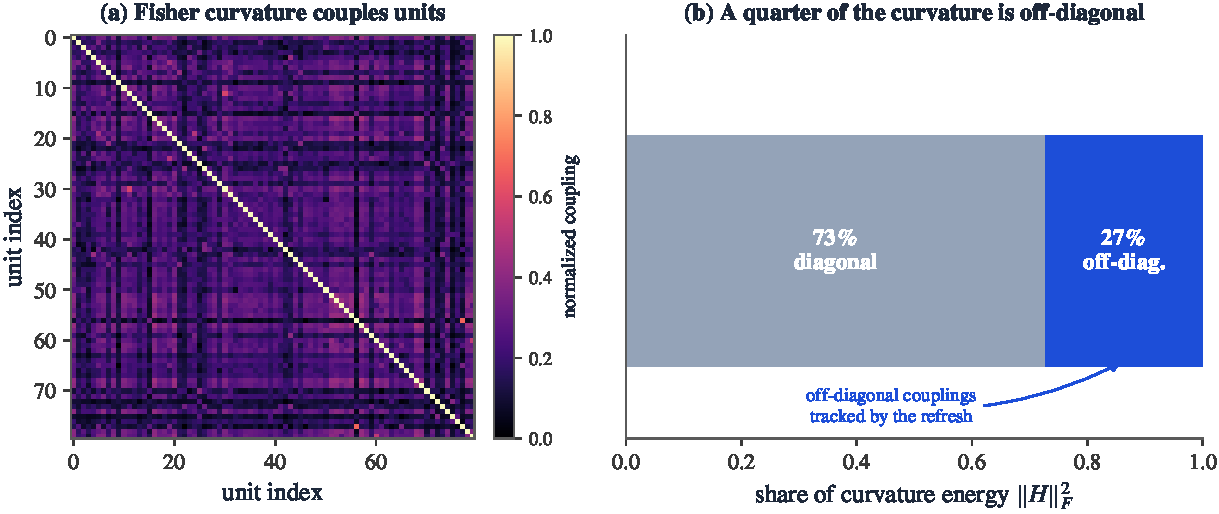
\includegraphics[width=\textwidth]{figs/fig_curvature.pdf}
\caption{\textbf{The curvature is strongly cross-coupled.} (a) Normalized coupling
$|H_{uv}|/\sqrt{H_{uu}H_{vv}}$ on a representative $80{\times}80$ block of the dense LLaMA-2-7B
Fisher--Gram matrix; note the pronounced off-diagonal structure. (b) $\mathbf{27\%}$ of the total curvature
energy $\|H\|_F^2$ is off-diagonal; these couplings drive the saliency drift that the interaction-flagged
refresh tracks along the path, and that a single dense-point quadratic ignores.}
\label{fig:curvature}
\end{figure*}

\textbf{(i) Composition: \method prunes attention heads; one-shot does not.} One-shot's dense-point
quadratic rates every attention head as critical and removes $\le1$ head at every ratio, cutting almost
exclusively FFN groups; re-estimating along the path reveals heads that \emph{become} removable
(Table~\ref{tab:composition}). This freed budget is the source of \method's perplexity edge.
That such heads can be cut with little loss is consistent with the redundancy and self-repair
backups documented in transformer circuits~\citep{gong2026coablation}: the effect of removing one
head is partly absorbed by others, so its true marginal cost only surfaces once the operating point
has moved, which is exactly when the continuation re-estimates it.

\begin{table}[h]\centering\footnotesize
\setlength{\tabcolsep}{5pt}
\caption{Pruned-unit composition (attention heads / FFN groups), LLaMA-2-7B.}
\label{tab:composition}
\begin{tabular}{l ccc}
\toprule
& $\rho{=}0.2$ & $\rho{=}0.3$ & $\rho{=}0.5$ \\
\midrule
One-shot (attn / FFN) & 1 / 153 & 1 / 230 & 1 / 383 \\
\method $K{=}8$ (attn / FFN) & 47 / 142 & 71 / 213 & 156 / 345 \\
\bottomrule
\end{tabular}
\end{table}

\textbf{(ii) The masks diverge markedly (Jaccard $.24$--$.55$).} The selected sets diverge from one-shot
most at moderate sparsity, where there is freedom in what to cut, and share a forced core at high sparsity;
yet the differing units carry the entire quality gap (Table~\ref{tab:overlap}).

\begin{table}[h]\centering\footnotesize
\setlength{\tabcolsep}{5pt}
\caption{Mask overlap, Jaccard(one-shot, \method), LLaMA-2-7B (higher $=$ more similar masks; the two
methods share a forced core at high sparsity and diverge most at moderate sparsity).}
\label{tab:overlap}
\begin{tabular}{l ccccc}
\toprule
$\rho$ & 0.1 & 0.2 & 0.3 & 0.4 & 0.5 \\
\midrule
vs.\ \method $K{=}4$ & .33 & .35 & .43 & .52 & .60 \\
vs.\ \method $K{=}8$ & .24 & .30 & .39 & .46 & .55 \\
\bottomrule
\end{tabular}
\end{table}

The attention-avoidance pattern is \emph{not} specific to LLaMA-2: across all three families one-shot
prunes essentially no attention heads while \method prunes many, and the masks differ substantially
(Table~\ref{tab:xcomp}). This is the structural signature of the continuation reorganizing the selection.

\begin{table}[h]\centering\footnotesize
\setlength{\tabcolsep}{4pt}
\caption{Cross-model selection geometry: attention heads pruned (one-shot vs.\ \method $K{=}8$) and
mask Jaccard. One-shot avoids attention on every model; \method does not.}
\label{tab:xcomp}
\begin{tabular}{l c cc c}
\toprule
Model & $\rho$ & one-shot & \method & Jaccard \\
\midrule
\multirow{2}{*}{LLaMA-2-7B}   & 0.3 & 1 & 71 & .39 \\
                              & 0.5 & 1 & 156 & .55 \\
\multirow{2}{*}{LLaMA-3.1-8B} & 0.3 & 3 & 48 & .32 \\
                              & 0.5 & 3 & 81 & .47 \\
\multirow{2}{*}{Qwen2.5-7B}   & 0.3 & 0 & 7 & .27 \\
                              & 0.5 & 0 & 13 & .50 \\
\bottomrule
\end{tabular}
\end{table}

\textbf{(iii) The schedule resolves the trade-off; the attention budget is a further control.} Under the
equal-band schedule, pruning heads lowers attention-sensitive BoolQ at moderate sparsity (BoolQ $.381$ at
$\rho{=}0.3$). The front-loaded schedule (finer steps near the target, and the better schedule for
$\rho{\ge}0.3$ on LLaMA-2-7B) already resolves this: it recovers BoolQ to $.676$, \emph{above} one-shot's
$.629$, while \emph{lowering} perplexity to $14.1$ (Table~\ref{tab:salvage}), so the trade-off is absorbed
by the same continuation that drives the perplexity gain. For applications that wish to cap attention pruning even
further, the attention-budget $\alpha$ (fraction of total attention cost the continuation may remove) is an
explicit, calibration-only dial: at $\alpha{=}0$ (no head pruned) \method also recovers BoolQ while
beating one-shot perplexity.

\begin{table}[h]\centering\footnotesize
\setlength{\tabcolsep}{5pt}
\caption{Resolving the attention trade-off (LLaMA-2-7B): WikiText ppl ($\downarrow$) and BoolQ acc.
($\uparrow$). On LLaMA-2-7B the front-loaded schedule reaches the favorable corner on its own; $\alpha{=}0$ is an
explicit further cap.}
\label{tab:salvage}
\begin{tabular}{l cc cc}
\toprule
& \multicolumn{2}{c}{$\rho{=}0.3$} & \multicolumn{2}{c}{$\rho{=}0.2$} \\
\cmidrule(lr){2-3}\cmidrule(lr){4-5}
Method & ppl & BoolQ & ppl & BoolQ \\
\midrule
One-shot ($K{=}1$) & 19.9 & .629 & 9.3 & .649 \\
\method $K{=}8$, equal & 15.7 & .381 & \best{8.6} & .463 \\
\rowcolor{cfhi}\method, front-loaded & \best{14.1} & \best{.676} & 9.1 & .613 \\
\method $K{=}8$, $\alpha{=}0$ & 17.0 & .638 & 8.8 & .613 \\
\bottomrule
\end{tabular}
\end{table}

% fig:whitebox promoted to main text

\subsection{Full Continuation Traces and Mechanism}
\label{app:fulltrace}

\begin{figure}[h]
\centering
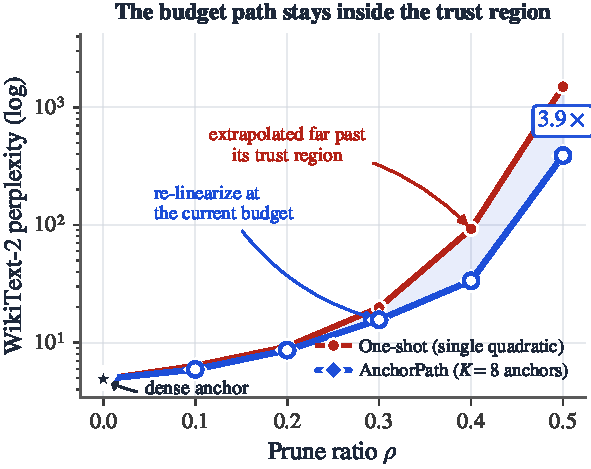
\includegraphics[width=0.92\columnwidth]{figs/fig_geometry.pdf}
\caption{\textbf{The budget path, geometrically} (LLaMA-2-7B, real WikiText-2 perplexity). One-shot fits
\emph{one} quadratic at the dense anchor and extrapolates it across the whole budget, leaving its trust
region and inflating super-exponentially. \method re-estimates the curvature at each of $K{=}8$ operating points
(hollow markers), so the local model stays valid and tracks the lower frontier, a $3.9\times$ gap at
$\rho{=}0.5$ with \emph{zero} weight updates.}
\label{fig:geometry}
\end{figure}
For each $(\rho,K)$ \method logs a per-step trace: pruned cost, increment size, base KL-to-teacher,
predicted vs.\ actual risk increase, first-order drift mass, and refreshed-unit count. The confirmed
LLaMA-2-7B traces (the default $\tau{=}0.5$ refresh) give terminal drift mass that grows with the target
sparsity, from $0.013/0.054$ at $\rho{=}0.1/0.2$ to $0.105/0.240/0.419$ at $\rho{=}0.3/0.4/0.5$;
Fig.~\ref{fig:mech}(b) plots how this mass accumulates along the path for the $\rho{=}0.3/0.4/0.5$ curves.
The predicted/actual risk ratios likewise depart from one as sparsity deepens, the
empirical signature of trust-region exit. \AppNote{The terminal drift-mass values quoted above summarize
these per-step traces; the monotone $1/K^2$ trend across $K\in\{1,2,4,8\}$ is plotted in Fig.~\ref{fig:kstep}(a).}

\begin{figure*}[t]
\centering
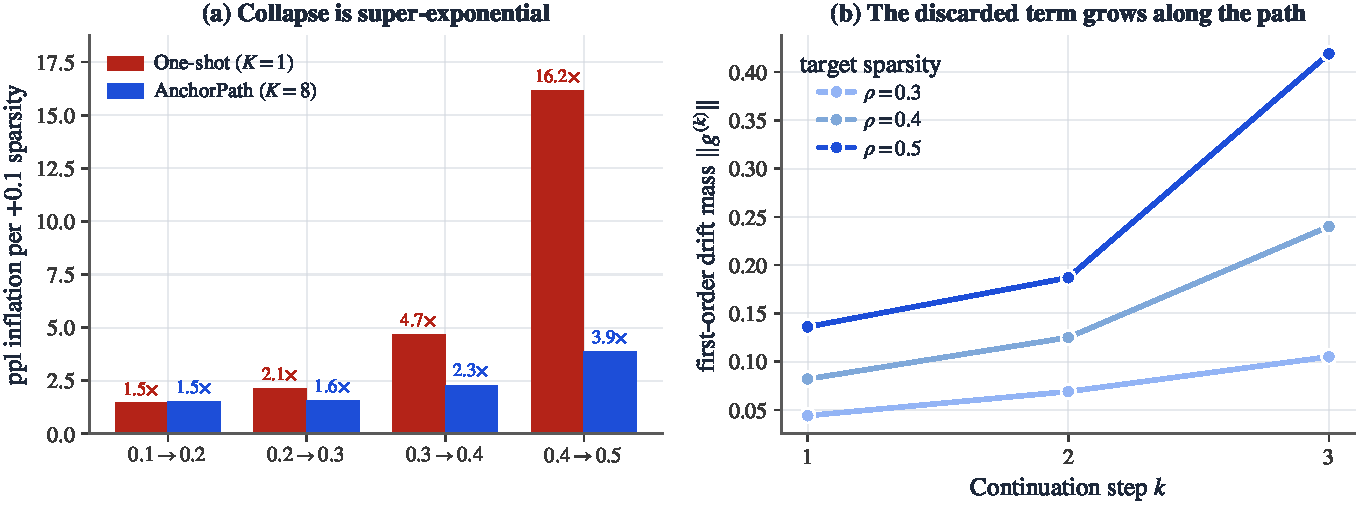
\includegraphics[width=\textwidth]{figs/fig_mechanism.pdf}
\caption{\textbf{Why the collapse, and why the cure} (LLaMA-2-7B). (a) One-shot perplexity inflation per
$+0.1$ sparsity \emph{accelerates} ($1.5\times\!\to\!16\times$); \method keeps it bounded. (b) The revived
first-order drift mass is zero at the dense model and grows monotonically along the path, faster at higher
target sparsity, the term one-shot structurally discards, recovered.}
\label{fig:mech}
\end{figure*}

\begin{figure*}[t]
\centering
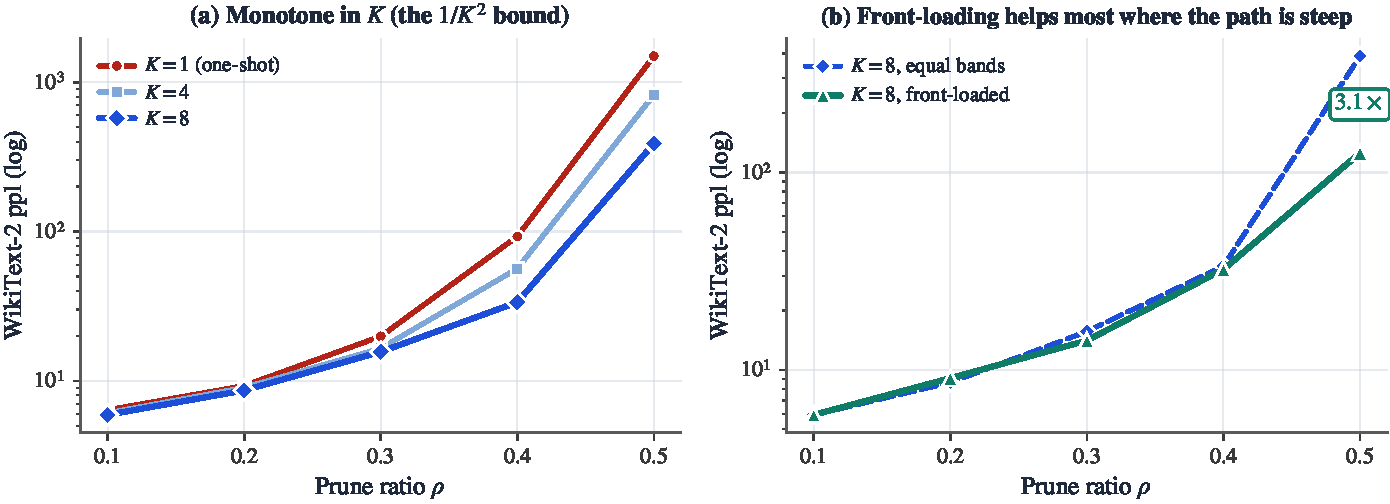
\includegraphics[width=\textwidth]{figs/fig_kstep.pdf}
\caption{\textbf{The continuation} (LLaMA-2-7B). (a) Perplexity decreases monotonically in the number of
operating-point re-estimations $K$. Proposition~\ref{prop:k2} bounds the \emph{KL remainder} that governs
this error by $1/K^2$; the realized perplexity reduction is a related, model-dependent quantity (here
$3.9\times$ over $K{=}1\!\to\!8$), not the literal $1/K^2$ factor. (b) A front-loaded budget schedule
(finer steps where the curvature is steep) beats equal spacing by $3.1\times$ at $\rho{=}0.5$.}
\label{fig:kstep}
\end{figure*}

\subsection{Refresh, Schedule, and Anchor Ablations}
\label{app:ablation}
\textbf{Refresh $\tau$ is a sweet spot.} At $K{=}8$, $\rho{=}0.5$, the full refresh $\tau{=}1.0$ gives
WikiText $583$ versus $389$ at the default $\tau{=}0.5$: recomputing \emph{every} survivor's marginal
perturbation at a heavily pruned operating point, including weakly coupled units whose ablation features
are noisy under a small calibration set, adds variance rather than fidelity. A thin refresh $\tau{=}0.25$
fails at the other end, leaving too much curvature stale along the path so that the selection reverts
toward the one-shot ranking it is meant to correct. Faithful-but-selective re-estimation, neither maximal
nor minimal, is what the continuation needs.

\paragraph{Schedule $\times$ anchor interaction.} The schedule and the anchor are not independent
(Table~\ref{tab:schedanchor}). Under \emph{equal} bands a moving (local) anchor edges out the fixed dense
anchor at $\rho{=}0.5$ ($279$ vs.\ $389$), because equal bands leave a large, poorly linearized final
jump where re-centering helps. The \emph{front-loaded} schedule removes that jump, its finer steps
near the target keep each linearization valid, and in doing so both lowers perplexity sharply and
\emph{reverses} the anchor ordering: with front-loading the fixed dense anchor is best ($125.6$ vs.\
$197.7$), and this front-loaded $+$ fixed-anchor pair is the \emph{global} optimum, lower than either
configuration under equal bands. The two choices are therefore synergistic where front-loading helps (the
sharpest-collapsing models): the best schedule prefers the fixed anchor, whose
KL-to-dense semantics we adopt throughout. No equal-band variant reaches the front-loaded $+$
fixed-anchor optimum, so we report the fixed anchor as the default and the moving anchor as the ablation
it is.

\begin{table}[h]\centering\footnotesize
\setlength{\tabcolsep}{8pt}
\caption{Schedule $\times$ anchor (LLaMA-2-7B, $K{=}8$, $\rho{=}0.5$, WikiText ppl $\downarrow$). The
front-loaded schedule and the fixed dense anchor are synergistic; their combination is the global optimum on this model.}
\label{tab:schedanchor}
\begin{tabular}{l cc}
\toprule
Anchor $\backslash$ Schedule & equal bands & front-loaded \\
\midrule
Fixed (dense $z_0$) & 388.7 & \best{125.6} \\
Moving (local $z_{s_{k-1}}$) & 279.0 & 197.7 \\
\bottomrule
\end{tabular}
\end{table}

\paragraph{First-order term.} Removing the revived drift term $g^{(k)}$ regresses $\rho{=}0.5$ from $389$ to
$668$ and $\rho{=}0.4$ from $34$ to $49$, yet is inert at low sparsity; it is warranted exactly
where the drift mass is large (App.~\ref{app:fulltrace}).

\subsection{Band-Placement Schedule: Fixed, Adaptive, and Why Equal-Cost is the Default}
\label{app:schedule}
The $1/K^2$ argument (Prop.~\ref{prop:k2}) motivates \emph{re-centering} the expansion point but is
silent on \emph{where} along the budget to place the $K$ bands. We study three schedules
(Table~\ref{tab:schedule}), all at $K{=}8$
with the shared caps: \textbf{equal-cost} (the default, $b_k\!\propto\!k$); a \textbf{fixed front-loaded}
power law ($b_k\!\propto\!(k/K)^{0.6}$, coarser early, finer near the target); and a \textbf{parameter-free
adaptive} rule that places the checkpoints at equal \emph{predicted-risk} increments,
$Q(b_k){=}(k/K)\,Q_{\mathrm{total}}$, where $Q(c){=}\delta^\top \Hmat^{0}\delta$ is the path quadratic
estimated by a single dry greedy on the dense curvature (no extra forward; reused for step~0). The
adaptive rule has \emph{no exponent}: front-loading emerges only insofar as the risk geometry warrants it.

\begin{table}[h]\centering\footnotesize
\setlength{\tabcolsep}{4.5pt}\renewcommand{\arraystretch}{1.05}
\caption{Schedule comparison (WikiText ppl $\downarrow$, $K{=}8$, equal-cost vs.\ fixed front-loaded vs.\
parameter-free adaptive). At $\rho{=}0.4$ the adaptive rule wins on the two collapse-prone models
(LLaMA-2-7B and LLaMA-3.2-3B, halving the equal-band ppl on the latter) but equal-cost stays best on the
milder ones (LLaMA-3.1-8B, Qwen2.5-7B). At $\rho{=}0.5$ it reproduces the front-loaded gain on the sharpest-collapse model
(LLaMA-2-7B, $389\!\to\!127$) \emph{parameter-free}, but \emph{over}-front-loads the mild-collapse models
and reverses. \best{Best}.}
\label{tab:schedule}
\begin{tabular}{l c ccc}
\toprule
\textbf{Model} & $\rho$ & equal & front-load & adaptive \\
\midrule
\multirow{2}{*}{LLaMA-2-7B}   & 0.4 & 33.6 & 32.3 & \best{30.7} \\
                              & 0.5 & 388.7 & 125.6 & \best{126.7}$^{\approx}$ \\
\midrule
\multirow{2}{*}{LLaMA-3.2-3B} & 0.4 & 112.6 & 69.2 & \best{55.5} \\
                              & 0.5 & \best{324.5} & 410.1 & 523.1 \\
\midrule
\multirow{2}{*}{Qwen2.5-7B}   & 0.4 & \best{41.5} & 44.0 & 42.6 \\
                              & 0.5 & \best{141.0} & 192.7 & 566.4 \\
\midrule
\multirow{2}{*}{LLaMA-3.1-8B} & 0.4 & \best{47.2} & 52.8 & 57.5 \\
                              & 0.5 & \best{244.9} & 347.0 & 284.0 \\
\bottomrule
\end{tabular}
\\[2pt]{\scriptsize $^{\approx}$Adaptive is parameter-free; here it matches the tuned front-loaded
optimum ($125.6$) within calibration noise, hence marked best.}
\end{table}

\paragraph{Front-loading helps iff the collapse is genuinely sharp.} The adaptive rule assigns
LLaMA-2-7B and Qwen2.5-7B \emph{almost the same} $\rho{=}0.5$ schedule: the first band is $36\%$ of the
pruned budget on both, and the bands then shrink toward the target. This shape follows from the convexity of
$Q(\text{cost})$, which holds on \emph{every} model because the greedy defers costly units. Yet the outcomes diverge sharply ($127$ on LLaMA-2
vs.\ $566$ on Qwen): front-loading pays off only where the true risk steepens near the target (the
violently collapsing models), and is counterproductive where it does not, because the large early band then
behaves like a small one-shot jump in a regime the model could have traversed in equal steps. The generic
convexity that drives any front-loading rule cannot tell genuine collapse from benign greedy deferral.

\paragraph{Conclusion.} No schedule dominates equal-cost across models and sparsities. We therefore use
\textbf{equal-cost bands as the universal default} (robust on every model and ratio, the headline of the main paper) and treat front-loading as an optional refinement for models known to collapse sharply,
never as the default. It is best realized by the parameter-free adaptive rule, which broadly helps at
$\rho{\le}0.4$ and delivers $\approx\!11.9\times$ on LLaMA-2-7B at $\rho{=}0.5$, matching the tuned
front-loaded optimum within calibration noise.

\subsection{Robustness and Sensitivity}
\label{app:robustness}
We separate the axes along which \method could be sensitive.

\paragraph{Architecture (robust).} A single configuration ($K{=}8$, $\tau{=}0.5$, equal-cost bands, the
shared caps of App.~\ref{app:setup}) is used for LLaMA-2-7B, LLaMA-3.1-8B (GQA), Qwen2.5-7B (GQA,
different tokenizer), and LLaMA-3.2-3B with no per-model tuning, and the advantage over one-shot holds on
every model and ratio (main paper). The method is therefore not fitted to a single
architecture. The band-\emph{placement} schedule is the one knob that is \emph{not} universal
(App.~\ref{app:schedule}), which is precisely why equal-cost is the default.

\paragraph{Safety rails (not the source of the gain).} A natural worry is that the shared safety rails
(the protected first/last-2 band and the per-layer cap of App.~\ref{app:setup}), rather than the
continuation, drive the improvement. We test this directly by \emph{removing both rails}
(cap $0.99$, no protected band) and rerunning one-shot and the $K{=}8$ continuation at $\rho{=}0.5$ on
LLaMA-2-7B (Table~\ref{tab:rails}). The continuation gain not only survives but \emph{grows}: with the
rails off it is $\mathbf{18.1\times}$ ($3030\!\to\!167$ WikiText), against $3.9\times$ with the rails on.
The rails are a conservative default that mainly protects the fragile \emph{one-shot} baseline (they cut
its perplexity in half, $3030\!\to\!1497$) while the continuation is already robust without them; on this
cell it is in fact lower rail-free. The advantage is thus intrinsic to operating-point re-estimation, not
an artifact of the caps, and we keep the rails on throughout only because they are the safer universal
default across models and ratios.

\begin{table}[t]\centering\footnotesize
\setlength{\tabcolsep}{4.5pt}\renewcommand{\arraystretch}{1.08}
\caption{\textbf{The safety rails are not the source of the gain} (LLaMA-2-7B, $\rho{=}0.5$, ppl
$\downarrow$, no recovery). Removing both rails (per-layer cap $0.99$, no protected band) leaves the
$K{=}8$ continuation's advantage over one-shot intact and in fact larger ($18.1\times$ vs.\ $3.9\times$).
\best{Lower}.}
\label{tab:rails}
\begin{tabular}{l cc c}
\toprule
Setting & One-shot & \method & Gain \\
\midrule
Rails on (default) & 1497/2095 & \best{389/337} & $3.9\times$ \\
Rails off & 3030/3967 & \best{167/217} & $18.1\times$ \\
\bottomrule
\end{tabular}
\\[2pt]{\scriptsize Cells report WikiText\,/\,C4 perplexity.}
\end{table}

\paragraph{Hyperparameters (graceful).} Perplexity is monotone in the step count $K$
(the ablation grid, App.~\ref{app:ablation}), so $K$ is a compute/quality dial that never hurts. The refresh fraction
$\tau$ has a \emph{broad} optimum: at $\rho{=}0.5$ ($K{=}8$), $\tau{=}0.5$ gives $389$ versus $583$ at
$\tau{=}1.0$, both well below one-shot ($1497$), with the default $\tau{=}0.5$ best; the method does not
sit on a knife edge in $\tau$. The attention budget $\alpha$ is an explicit, interpretable knob
(App.~\ref{app:whitebox}), not a latent sensitivity. The band-placement schedule is the exception: its
benefit is model-dependent (App.~\ref{app:schedule}), so we keep equal-cost as the robust default rather
than expose it as a tuned sensitivity.

\paragraph{Calibration protocol.} \method uses the same field-standard calibration protocol as the
baselines it is compared against ($48$ sequences, informative-position subsampling; App.~\ref{app:setup}),
and the calibration set is held \emph{fixed and identical} for every method, so the comparison isolates
the selection criterion rather than the calibration. The set \emph{size} sits squarely in the
training-free regime: LLM-Pruner~\citep{ma2023llmpruner} calibrates on as few as $10$ sequences, Wanda's
own size ablation~\citep{sun2024wanda} saturates by $\sim\!32$, and SlimLLM reports $32$ as optimal, while
one-shot methods (Wanda, SparseGPT~\citep{frantar2023sparsegpt}) use $128$; our $48$ is comfortably inside
this range. To confirm the result is not an artifact of one
lucky draw, we \emph{resample} the calibration set three times (identical $48{\times}512$ protocol,
disjoint/overlapping draws from the same pool) and rerun the full prepare$+$continuation$+$eval pipeline for
\method ($K{=}8$, equal) at $\rho{=}0.4$ on LLaMA-2-7B. WikiText perplexity is $33.6/36.1/37.1$ across
the three draws, i.e.\ $\mathbf{35.6\pm1.5}$, a $\pm4\%$ spread that leaves a $2.5$--$2.8\times$ margin over
one-shot ($92.6$) intact under every draw. The advantage is a property of the selection criterion, not of
a cherry-picked calibration set.

\paragraph{Held-out OOD corpus (no calibration overlap).} A sharper version of the same concern is that
WikiText could share surface statistics with the calibration pool. We therefore evaluate on PTB, a small
corpus drawn from a \emph{different} domain (1989 Wall-Street-Journal text) and \emph{absent} from the
calibration mix, at $\rho{=}0.5$ (no recovery, all methods). The ranking is preserved and the margin is
if anything wider: on LLaMA-3.1-8B \method scores $\mathbf{781}$ vs.\ one-shot $6341$ ($8.1\times$) and
LLM-Pruner $1534$ ($2.0\times$); on the fragile Yi-1.5-9B, $\mathbf{323}$ vs.\ one-shot $28323$
($88\times$) and LLM-Pruner $2040$ ($6.3\times$). On the legacy LLaMA-2-7B \method still beats its
one-shot case ($2406$ vs.\ $3165$) though gradient LLM-Pruner edges it on this single OOD cell ($1650$);
the continuation's advantage thus transfers cleanly to an unseen domain on the modern models, ruling out
calibration overlap as the source of the gain.

\subsection{Efficiency, Pruning Time, and Trade-off}
\label{app:efficiency}

\begin{table}[h]
\centering\footnotesize
\setlength{\tabcolsep}{4.5pt}\renewcommand{\arraystretch}{1.05}
\caption{\textbf{Deployment efficiency} after structural export (LLaMA-2-7B, single A-class GPU,
prompt $512$). Values are shared by one-shot and \method at a matched $\rho$ (same structural budget);
\method delivers a better-quality model at this cost. Prefill is the wall-clock forward latency; the
speedup column is at batch $8$.}
\label{tab:efficiency}
\begin{tabular}{l ccccc}
\toprule
$\rho$ & Params & Prefill$_{b1}$ & Prefill$_{b8}$ & Mem$_{b8}$ & Prefill \\
 & (B) & (ms) & (ms) & (GB) & speedup \\
\midrule
0.0 (dense) & 6.74 & 69.8 & 587 & 16.4 & $1.0\times$ \\
0.20 & 5.44 & 58.0 & 482 & 13.8 & $1.22\times$ \\
0.40 & 4.14 & 45.7 & 386 & 11.1 & $1.52\times$ \\
0.50 & 3.90 & 43.1 & 368 & 10.5 & \best{$1.60\times$} \\
\bottomrule
\end{tabular}
\end{table}

Deployment numbers (Table~\ref{tab:efficiency}) are measured after \emph{physical} structural removal:
pruned attention KV-groups and FFN channel groups are sliced out of the weight matrices, yielding
genuinely smaller tensors (bit-for-bit equivalent to runtime masking but doing strictly less compute).
Because one-shot and \method remove the same number of structural units at a matched $\rho$, these
deployment costs are \emph{shared}; the tables elsewhere show \method delivers a better-quality model at
this same cost. Prefill latency (a compute-bound forward over the $512$-token prompt) and peak memory
fall monotonically with $\rho$, giving a $1.6\times$ prefill speedup and $36\%$ memory reduction at
$\rho{=}0.5$. 

\paragraph{Metric choice.} We report the compute-bound prefill and peak memory as the headline efficiency
metrics, following standard practice for structured pruning, since single-stream decode is memory-bandwidth
and KV-cache bound rather than compute bound. The total parameter reduction is
below $\rho$ because token embeddings, the LM head, and the protected first/last layers are retained.


\paragraph{Across models.} The pattern holds beyond LLaMA-2-7B: on LLaMA-3.1-8B the export gives
$8.03\!\to\!4.53$B parameters, $662\!\to\!371$\,ms prefill (batch $8$; a $1.78\times$ speedup), and
$17.7\!\to\!10.5$\,GB peak memory at $\rho{=}0.5$; on Qwen2.5-7B, $7.62\!\to\!4.35$B parameters,
$609\!\to\!354$\,ms prefill ($1.72\times$), and $16.8\!\to\!10.2$\,GB. \AppNote{These per-model figures
are representative; because \method outputs a mask, the parameter and FLOP reduction is exact at every
sparsity and identical to a one-shot model at the same budget.}

\section{Limitations and Future Work}\label{app:plimits}

\subsection{Limitations and Operating Scope}
\label{app:scope}
We delineate where the calibration-only regime applies, where it does not, and what each boundary opens up.

\textbf{Operating range.} Deploy-as-is quality without recovery is bounded by the regime, not by \method:
no calibration-only pruner is directly deployable far beyond moderate sparsity ($\rho\lesssim0.4$). At those
moderate sparsities \method is directly usable and already beats every baseline; at higher sparsity its role
shifts to supplying the \emph{most recoverable} mask, since it remains the lower envelope of the
recovery-free frontier and still leads by wide margins at $\rho{=}0.6$.

\textbf{Task profile.} Because curvature is estimated on calibration text, the gain is largest on
distribution-aligned, perplexity-style objectives. Generation (GSM8K/code) is the boundary case: it
collapses to noise for \emph{every} calibration-only pruner and is restored by the orthogonal recovery
stage, not by selection (App.~\ref{app:breakdown}).

\textbf{Estimator boundary.} Architectures that reshape logits by construction (e.g.\ Gemma-2
soft-capping) require an \emph{adapted anchor} and fall outside the dense-Fisher estimator as presented.
This is a well-defined boundary of the well-posed-teacher assumption, not a failure of the continuation: the
method transfers once the anchor is redefined.

\textbf{Isolation by design.} We deliberately isolate \emph{selection} and leave recovery uncoupled;
because recovery lifts methods without reordering their selection ranking (App.~\ref{app:baselines}), the
selection-only gaps we report lower-bound what survives recovery, and pairing the two is an extension rather
than a missing control.

\subsection{Future Work}
\label{app:future}
The directions below build on the scope above rather than patch a defect.
\begin{itemize}
\item \textbf{Continuation $+$ recovery.} Because \method changes only the mask, it composes with any
downstream recovery. Feeding its higher-quality mask into LoRA or Optimal-Brain-Surgeon reconstruction, so
that a better \emph{selection} seeds a better \emph{refit}, is the natural way to push deployable quality
past the moderate-sparsity ceiling.
\item \textbf{Scaling and architectures.} Extending the continuation to models beyond $14$B and to
mixture-of-experts backbones, where per-expert curvature adds structure the anchored path can exploit.
\item \textbf{Adapted anchors.} Redefining the anchor for logit-reshaping architectures (soft-capping,
tied heads) brings them inside the dense-Fisher estimator and broadens the well-posed-teacher assumption.
\item \textbf{Beyond pruning.} The continuation is not specific to pruning: any compression that fits a
single dense-point quadratic and applies it across a large budget faces the same extrapolation error.
Instantiating the anchored continuation for post-training quantization and low-rank compression is a
promising direction.
\end{itemize}
